
\chapter{Background and State of the Art}
\label{ch:sota}

This chapter establishes the theoretical foundations of this work and reviews
the relevant prior literature. We begin by introducing the core concepts and
notation used throughout the thesis, covering recurrent and spiking neural
networks, eligibility traces, and the reinforcement learning framework. We
then survey the state of the art in training recurrent networks online,
tracing the progression from classical backpropagation through time to eligibility-based and perturbation-based methods, and concluding with
the existing approaches to online reinforcement learning in spiking networks
that most directly motivate the contributions of this work.

% ============================================================
\section{Preliminaries and Notation}
\label{sec:preliminaries}

This section briefly introduces the core concepts and notation used
throughout this work. It is intended as a quick reference. Each topic is developed in greater depth in the
sections that follow.

\subsection{Models of Neural Computation}

We consider \emph{recurrent neural networks} (RNNs), networks that maintain
an internal hidden state $h_t \in \mathbb{R}^n$ updated at each timestep as
$h_t = f(h_{t-1}, x_t; \theta)$, allowing past inputs to influence future
outputs. A special case of particular interest here is \emph{spiking neural
networks} (SNNs), in which neurons communicate through discrete binary events
$z^t_j \in \{0, 1\}$ instead of the traditional rate-based networks approach of applying continuous activation functions. Each neuron
maintains a membrane potential $v^t_j$ that integrates incoming spikes over
time and resets upon crossing a firing threshold $v_{th}$. This
discontinuous spike generation mechanism prevents standard gradient-based
optimization from being applied directly; the techniques used to overcome
this limitation are discussed in the following sections.

\subsection{Temporal Credit Assignment}

A fundamental difficulty in training recurrent networks is that a parameter
change at time $t$ may only manifest in the loss $E$ many steps later,
creating complex temporal dependencies in $\frac{\mathrm{d}E}{\mathrm{d}\theta}$.
Determining which past activities were responsible for a present outcome is
known as the \emph{temporal credit assignment problem}, and it is the central
challenge addressed by every method reviewed in this chapter.
\emph{Eligibility traces} $e^t_{ji}$ are per-synapse variables that maintain
a local, forward-in-time record of how weight $W_{ji}$ has shaped recent
neural activity. They form the backbone of the online learning rules
developed throughout this work, and their key advantage is that they can be
computed incrementally without storing the full history of network states.

\subsection{Reinforcement Learning}

An agent interacts with an environment by following a policy
$\pi(a \mid s)$, collecting rewards $R_t$ with the goal of maximizing the
discounted return $G_t = \sum_{k \geq 0} \gamma^k R_{t+1+k}$. The
\emph{state-value function} $v_\pi(s) = \mathbb{E}_\pi[G_t \mid S_t = s]$
captures the expected return from each state and satisfies the Bellman
consistency condition
\begin{equation}
    v_\pi(s) = \mathbb{E}_\pi\!\left[R_{t+1} + \gamma\, v_\pi(S_{t+1})
    \mid S_t = s\right].
\end{equation}
The degree to which this condition is violated at any given step is measured
by the \emph{temporal-difference (TD) error},
\begin{equation}
    \delta_t = R_{t+1} + \gamma V_{t+1} - V_t,
\end{equation}
which serves as the primary online learning signal throughout this work.

\subsection{Notation Summary}

\begin{table}[h]
\centering
\begin{tabular}{ll}
\toprule
\textbf{Symbol} & \textbf{Meaning} \\
\midrule
$h_t$                        & Hidden state at time $t$ \\
$x_t$                        & Input at time $t$ \\
$z^t_j$                      & Spike output of neuron $j$ at time $t$ \\
$v^t_j$                      & Membrane potential of neuron $j$ at time $t$ \\
$v_{th}$                     & Spike threshold \\
$\alpha$                     & Membrane decay factor \\
$\mathcal{F}_\alpha$         & Exponential decay filter with parameter $\alpha$ \\
$W_{ji}$                     & Synaptic weight from neuron $i$ to $j$ \\
$e^t_{ji}$                   & Eligibility trace for synapse $ji$ at time $t$ \\
$L^t_j$                      & Learning signal for neuron $j$ at time $t$ \\
$E$                          & Loss function \\
$S_t,\ A_t,\ R_t$            & RL state, action, and reward at time $t$ \\
$\pi(a \mid s)$              & Stochastic policy \\
$G_t$                        & Discounted return at time $t$ \\
$\gamma$                     & Discount factor \\
$V_t$                        & Value estimate at time $t$ \\
$\delta_t$                   & Temporal-difference error \\
$\epsilon_j,\ \epsilon_{ji}$ & Perturbation at neuron $j$ or synapse $ji$ \\
\bottomrule
\end{tabular}
\caption{Summary of notation used throughout this work.}
\label{tab:notation}
\end{table}

% ============================================================
\section{Learning in Recurrent Neural Networks}
\label{sec:rnn-learning}

Having established the basic framework, we now turn to the problem of
training recurrent networks. This section describes the dominant approach,
Backpropagation Through Time, and explains why its structural requirements
make it poorly suited to the online, continuous-interaction settings that
motivate this work.

Recurrent Neural Networks (RNNs) have long been recognized as harder to
train than regular feedforward networks
\citep{learningLongTermHard, Werbos1990BackpropagationTT}. Recurrence
introduces temporal dynamics and dependencies into the network; past neural
activations influence current states, which significantly complicates the
process of gradient estimation. In feedforward networks, all causal
dependencies are separated by the topological ordering of the network.
This allows the backpropagation algorithm to accumulate gradient information
locally at each neuron by propagating errors backward through the network
layers. Although backpropagation is not online in time, it does not require
access to future network states beyond the current forward pass.

In recurrent networks, however, temporal dependencies prevent such a
separation. The effect of a neural activation at time $t$ may only become
apparent at much later times, meaning that full gradient computation requires
access to future network states.

\subsection{Backpropagation Through Time}

The canonical solution to the previously stated problem is Backpropagation Through Time (BPTT) \citep{Werbos1990BackpropagationTT}. The main idea is to convert the recurrent network into a feedforward network by unrolling it, making each timestep a "layer" of neurons that get their input from the previous state of the neurons, and influence the next "layer" in the next timestep. 

The unrolled network then could be understood as a flexible in size network with shared weights between all layers. BPTT is able to compute the exact gradient in RNNs, but, only if all network states through time have been stored. To "see" the effect of an activation of a neuron, the backpropagation algorithm needs to access the information in the future, where it can see the effect in the loss function and propagate backwards the loss information. 

We can see then, that to observe how the temporal dynamics of an RNN at the timestep $t$ influence the loss at $t+n$ we need to store all network states from $t$ to $t+n$, leading to memory requirements that scale linearly with the sequence length.

\subsection{Limitations for Online Learning}

Even though BPTT has been highly successful in practice, its need to store past activities and to perform backward passes over complete sequences prevents it from being a true online algorithm, especially in continuous data stream settings \citep{OSTL}. When dealing with very long or unbounded sequences, the history used by BPTT must be truncated, which introduces additional limitations. As discussed in \citet{OSTL}, citing earlier work by
\citet{WilliamsZipser1995} and \citet{Jaderberg2016}:

\begin{quote}
Truncated BPTT (TBPTT) reduces the amount of information that needs to be stored by splitting the input stream
into shorter segments and by updating the parameters of the
network after each segment (Williams and Zipser 1995).
However, it still leads to so-called system-locking problems (Jaderberg et al. 2016), because the parameter updates
can only be computed after the last input of each segment
has been processed. In addition, TBPTT encounters learning
deficiencies in tasks where there are long time lags between
the network activity and the feedback from the environment.
\end{quote}

These limitations make TBPTT poorly suited for strictly online learning scenarios and tasks with long temporal dependencies.

\section{Online Learning in Recurrent Systems}

\subsection{Requirements for Online Learning}

We understand online learning as a learning paradigm in which model
parameters are updated incrementally as data is processed, without
requiring access to future inputs or the storage of complete past
trajectories \citep{eprop2020, UORO}. In recurrent systems, this implies that learning updates should be computed at each timestep using information locally available at that time, making online learning particularly suitable for continuous and potentially unbounded data streams.

This definition is intentionally strict with respect to which learning algorithms it includes. For instance, Backpropagation Through Time and its truncated variants rely on storing past network states over a temporal window and performing backward passes to apply the chain rule, which prevents parameter updates from being computed strictly at the current timestep. As a result, such methods do not satisfy the requirements of online learning as defined here.

Part of the motivation for adopting this definition is to move toward learning mechanisms that more closely resemble those observed in biological systems, while also benefiting from properties such as constant memory usage over time, low-latency updates, and suitability for continuous, non-episodic interaction with dynamic environments. 

\subsection{Real-Time Recurrent Learning}

Real-Time Recurrent Learning (RTRL), introduced by \citet{RTRL}, provides a principled solution to the online learning problem in recurrent neural networks by computing exact gradients in a purely forward-in-time manner. In contrast to Backpropagation Through Time, RTRL does not require storage of past activations or a backward pass through time. Instead, it incrementally maintains derivatives of the hidden state with respect to the network parameters as the sequence unfolds.

Consider a recurrent neural network with hidden state $h_t$ and parameters $\theta$. RTRL maintains, at each time step $t$, the quantity:
\[
\frac{\partial h_t}{\partial \theta},
\]
which represents how changes in the parameters influence the current hidden state. This quantity is updated recursively using the chain rule as new inputs arrive. If we denote the recurrent update as $h_t = f(h_{t-1}, x_t; \theta)$, then the derivative evolves according to:
\[
\frac{\partial h_t}{\partial \theta}
=
\frac{\partial f}{\partial h_{t-1}} \frac{\partial h_{t-1}}{\partial \theta}
+
\frac{\partial f}{\partial \theta}.
\]

This recursion ensures that the influence of all past parameter changes is continuously propagated forward in time, enabling exact gradient computation at each timestep without revisiting past states.

However, the main limitation of RTRL lies in its computational cost. For a network with $n$ hidden units, the Jacobian $\frac{\partial h_t}{\partial \theta}$ is a three-dimensional tensor, leading to a naive computational complexity of $O(n^4)$ per timestep and memory complexity of $O(n^3)$. This arises from the need to track how every parameter affects every hidden unit through time, and how these effects interact multiplicatively through recurrent connections.

In practice, this cost makes standard RTRL infeasible for networks of realistic size. As a result, much of the modern literature focuses on approximations that reduce this complexity while preserving the online nature of the algorithm. Examples include Unbiased Online Recurrent Optimization (UORO) \citep{UORO}, which reduces the rank of the Jacobian estimate, and more recent structured approximations such as Kronecker-Factored RTRL (KF-RTRL), which exploit low-rank structure in the recurrent dynamics \citep{eprop2020}.

Despite its computational limitations, RTRL remains theoretically important as it represents the gold standard for online gradient computation in recurrent systems and provides the foundation for many biologically plausible and memory-efficient approximations. In particular, it highlights the key idea that learning in recurrent networks can be decomposed into (i) local eligibility traces capturing temporal credit assignment and (ii) learning signals that modulate these traces, a perspective that is further developed in modern approaches such as e-prop.

\section{Gradient Estimation with E-prop}
\label{sec:e-prop}
E-prop (eligibility propagation  \cite{eprop2020}) provides a framework for online learning in recurrent neural networks that addresses the limitations of both BPTT and RTRL. Instead of attempting to compute exact gradients through time or maintaining full Jacobians of the network dynamics, e-prop leverages a structural decomposition of the gradient into components that can be computed locally and components that carry information about the loss.

This perspective leads to learning rules in which synaptic updates are expressed as the interaction between locally computable eligibility traces and neuron-specific learning signals. The resulting algorithm operates in a strictly forward-in-time manner, requires constant memory with respect to sequence length, and remains applicable to networks with complex temporal dynamics.

In this section, we introduce e-prop in the context of spiking recurrent neural networks, where its interpretation in terms of local synaptic variables and global modulatory signals becomes particularly natural. We then derive the decomposition underlying e-prop and discuss practical variants that enable efficient and scalable learning.

\subsection{Spiking Recurrent Neural Networks}

Inspiration in biological systems has proven to be a good heuristic for system design. In this case, spiking recurrent neural networks (SRNNs) try to mimic the observed dynamics of the brain, where neurons communicate with pulses. Time is an intrinsic part of their design, even without recurrent connections the way they integrate past activations of connected networks enable them to remember information from many time steps ago. Recurrent connections then let the network not only remember the previous activations but "act" on them through time. It is clear then that the main tasks that these networks try to solve are time-related tasks, which involve temporal credit assignment.

The derivation in \cite{eprop2020} is made with SRNNs in mind, so it is important for us to understand how they define them and the additional problems they present. To quote \cite{eprop2020}:
\begin{quote}
We consider the arguably most prominent model for spiking neurons in the brain, the leaky integrate-and-fire (LIF) neurons, where spikes that arrive from other neurons through synaptic connections are multiplied with the corresponding synaptic weight, and are linearly integrated by a leaky membrane potential. The neuron fires—i.e., emits a spike—when the membrane potential reaches a firing threshold....Spikes are modeled as binary variables  $z^t_j$ that assume value $1$ if neuron $j$ fires at time $t$, otherwise value $0$. It is common in models to let $t$ vary over small discrete time steps, e.g., of $1\ ms$ length.  
\end{quote}
The dynamics of LIF neurons are defined by the equations
\begin{equation}
v^{t+1}_j = \alpha v^t_j + \sum_{i \neq j} W^{rec}_{ji} z^t_i + \sum_i W^{in}_{ji} x^{t+1}_i - z^t_jv_{th}
\end{equation}
\begin{equation}
z^t_j=H(v^t_j-v_{th})
\end{equation}
which can be interpreted as a leaky integration process where the membrane potential
retains a fraction $\alpha v^t_j$ of its previous value, accumulates incoming spikes
through the recurrent and input weights, and is reset by $v_{th}$ whenever the neuron emits a spike.

In addition, a refractory period is imposed by fixing $z^t_j = 0$ for a short interval after each spike. This constraint can be interpreted as a simple mechanism to regularize the neuron dynamics preventing arbitrarily high firing frequencies. As a result, the network is encouraged to represent information in its temporal structure, which improves stability significantly. 

Quoting \cite{eprop2020} again:
\begin{quote}
    $W^{rec}_{ji}$ ($W^{in}_{ji}$) is the synaptic weight from network (input) neuron $i$ to neuron $j$. The decay factor $\alpha$ in (6) is given by $e^{-\delta t/\tau_m}$ , where $\tau m$ (typically 20 ms) is the membrane time constant. $\delta t$ denotes the discrete time step size, which is set to $1 ms$ in our simulations. H denotes the Heaviside step function....the neurons membrane potential is reduced by a constant value after an output spike, which relates our model to the spike response $model^{53}$. To introduce a simple model of neuronal refractoriness, we further assume that $z^t_j$ is fixed to $0$ after each spike of neuron $j$ for a short refractory period of $2–5 ms$ depending on the simulation.
\end{quote}

To enhance the network capabilities we can also let the activation threshold update over time at a slower time scale than the integration dynamics, this type of neuron is called adaptive leaky integrate-and-fire (ALIF). These neurons have a two dimensional internal state $h^t_j \defeq \left[ v^t_j, a^t_j\right]$. Their threshold potential $A^t_j$ behaves in the following way:
\begin{equation}
A^t_j = v_{th} + \beta a^t_j
\end{equation}
\begin{equation}
a^{t+1}_j=\rho a^t_j + z^t_j
\end{equation}
Then the spikes take into account the threshold potential:
\begin{equation}
z^t_j=H(v^t_j-A^t_j)
\end{equation}
These network dynamics are not differentiable due to the discontinuous spike generation function. In particular, the derivative of $z^t_j = H(v^t_j - A^t_j)$ with respect to the membrane potential $v^t_j$ is zero almost everywhere and undefined at the threshold. As a result, standard gradient-based optimization cannot be applied directly.


To address this issue, surrogate gradient methods replace this non-existent
derivative with a smooth approximation \citep{Neftci2019Surrogate}. Concretely, a pseudo-derivative $\psi^t_j \approx \frac{\partial z^t_j}{\partial v^t_j}$ is introduced, which provides a non-zero gradient in a small region around the firing threshold. The pseudo-derivative used in \cite{eprop2020} is defined as:
\begin{equation}
\psi^t_j = \frac{1}{v_{th}}\gamma_{pd}\max \left( 0, 1- \left|\frac{v^t_j - A^t_j}{v_{th}} \right|\right)\ ;\ \text{where } \gamma_{pd}=0.3
\end{equation}
This function is non-zero only when the membrane potential $v^t_j$ is close to the threshold $A^t_j$, and vanishes otherwise. Intuitively, this means that gradients are propagated only when the neuron is close to firing, assigning credit to inputs that influenced the spike, or prevented it from happening.

During the refractory period, $\psi^t_j$ is set to $0$, since the neuron is prevented from firing and its dynamics are externally constrained. This ensures that no gradient is propagated during this interval, maintaining consistency between the forward dynamics and the learning rule.

\begin{figure}[h]
    \centering
    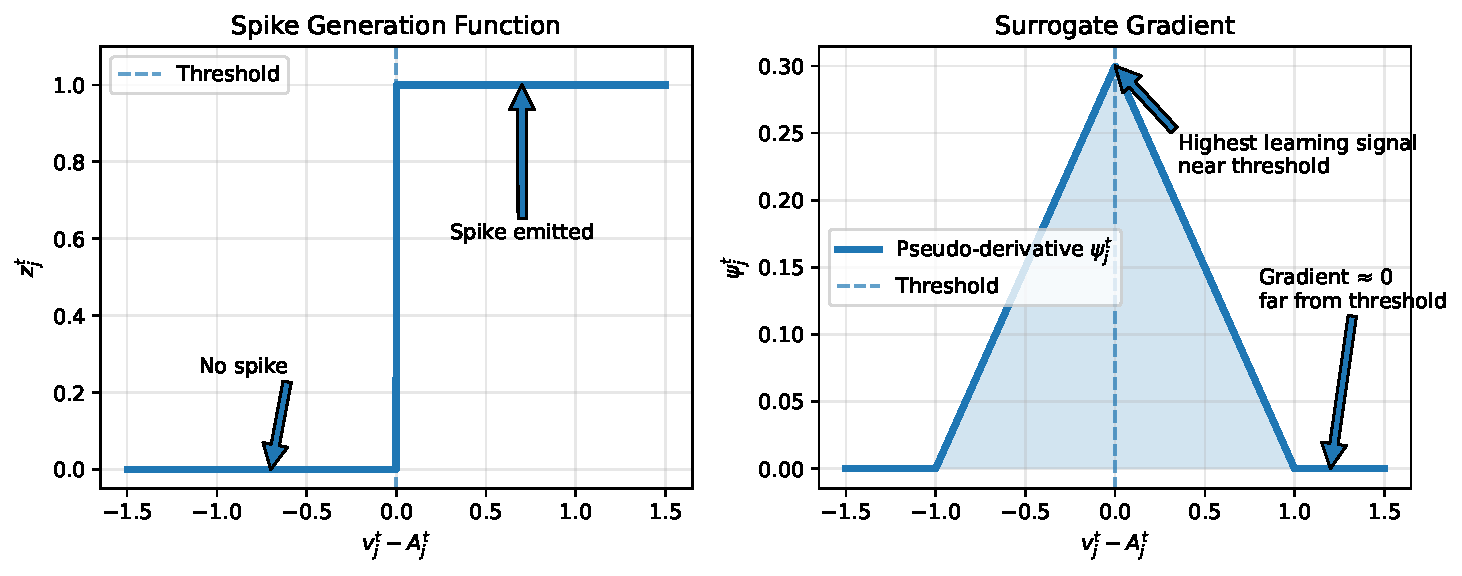
\includegraphics[width=1.0\linewidth]{images/spiking_function_dynamics.pdf}
    \caption[Spike generation and surrogate gradient]{Spiking function dynamics and surrogate gradient. Left: spike generation in a leaky integrate-and-fire neuron, modeled by the Heaviside function. A spike is emitted when the membrane potential exceeds the firing threshold. Right: pseudo-derivative used during learning. Because the true derivative of the Heaviside Step function is zero almost everywhere and undefined at threshold, it is replaced by a triangular surrogate gradient. The surrogate assigns the largest learning signal to membrane potentials close to threshold, where small input changes can alter the spiking decision, while activity far from threshold receives negligible credit.}
    \label{fig:spiking-function-dynamics}
\end{figure}

\clearpage
\subsection{E-prop: Separation of Local gradient and Loss gradient}

The key innovation of \cite{eprop2020} is the proof that the gradient $\frac{\mathrm{d}E}{\mathrm{d} W_{ji}}$ can be represented as a decomposition of two parts:
\begin{equation} \label{eq:epropDecomposition}
\sum_t \frac{\mathrm{d}E}{\mathrm{d}z^t_j} \cdot \left[ \frac{\mathrm{d}z_j^t}{\mathrm{d}{W_{ji}}} \right]_{local} 
\end{equation}

Quoting \cite{eprop2020}:
\begin{quote}
This local gradient is defined as a sum of products of partial
derivatives concerning the hidden state $h^t_j$ of neuron $j$ at time $t$ and preceding time steps, which can be updated during the
forward computation of the RNN by a simple recursion (Eq.(14)). This term $\left[ \frac{\mathrm{d}z_j^t}{\mathrm{d}{W_{ji}}} \right]_{local}$ is not an approximation. Rather, it collects the maximal amount of information about the network gradient $\frac{\mathrm{d}E}{\mathrm{d} W_{ji}}$ that can be computed locally in a forward manner. Therefore, it is the key-factor of e-prop. As it reduces for simple neuron models—whose internal state is fully captured by its membrane potential—to a variation of terms that are commonly referred to as eligibility traces
\end{quote}
They define the eligibility traces of the weight connecting the pre-synaptic neuron $i$ and the post-synaptic neuron $j$ ($e^t_{ji}$), and the loss signal for the output neuron $j$ ($L^t_j$) as:
$$
    e^t_{ji} \defeq \left[ \frac{\mathrm{d}z_j^t}{\mathrm{d}{W_{ji}}} \right]_{local}
    L^t_j \defeq \frac{\mathrm{d}E}{\mathrm{d}z^t_j} 
$$

The term $e^t_{ji}$ is referred to as the \emph{eligibility trace} because it captures the causal effect of the synapse from neuron $i$ to neuron $j$ on the firing of neuron $j$ at time $t$. In contrast, $L^t_j$ acts as a \emph{learning signal}, indicating the causal effect of the spike of neuron $j$ at time $t$ on the loss. This definition yields the following representation for the weights gradient:
\begin{equation} \label{eq:SumLossEtraces}
\frac{\mathrm{d}E}{\mathrm{d}W_{ji}} = \sum_t L^t_je^t_{ji}
\end{equation}

Having the weights' gradient, it is clear how to define an update rule that will minimize $E$ in an online manner, we have to update the weights at time $t$ proportional to $-L^t_je^t_{ji}$. If we use this definition by itself, we could not compute the actual weights gradient online; that is because $L^t_j$ is influenced by the spikes from previous time steps through recurrent connections in the network. To relax this requirement, $L^t_j$ is replaced by the partial derivative $\frac{\partial E}{\partial z^t_j}$, which only takes into account the direct influence of the spikes $z^t_j$.

\begin{figure}[h]\label{fig:EpropComputationFlow}
    \centering
    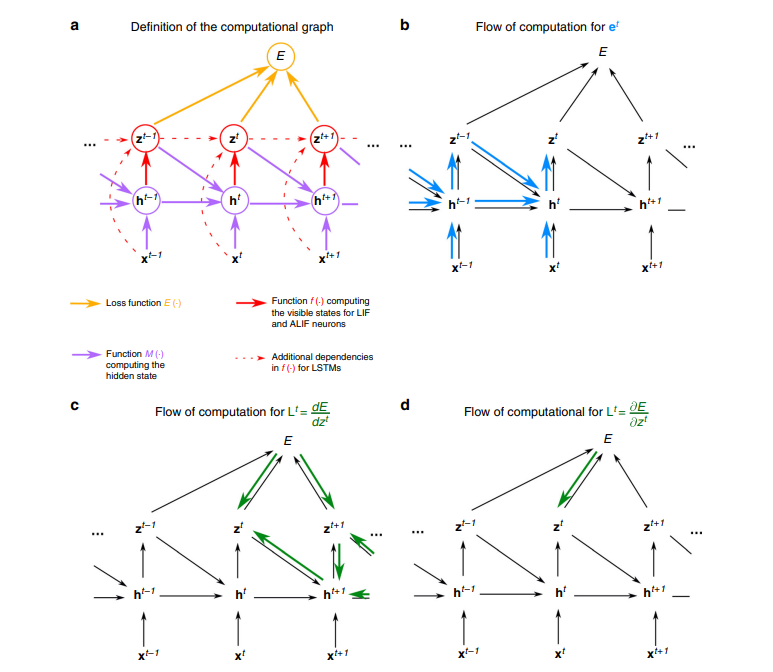
\includegraphics[width=1.0\linewidth]{images/EpropComputationFlow.png}
    \caption[E-prop computational graph (Bellec et al., 2020)]{%
    \textbf{Original caption from \citet{eprop2020}:} ``\textbf{Fig. 6 Computational graph and gradient propagations}. $\textbf{a}$ Assumed mathematical dependencies between hidden neuron states $\textbf{h}^t_j$ , neuron outputs $\textbf{z}^t$, network inputs $\textbf{x}^t$, and the loss function $E$ through the mathematical functions $E( \cdot ), M( \cdot ), f( \cdot )$ are represented by colored arrows. \textbf{b–d} The flow of computation for the two components $\textbf{e}^t$ and $\textbf{L}^t$ that merge into the loss gradients of Eq. (3) can be represented in similar graphs. \textbf{b} Following Eq. (14), the flow of the computation of the eligibility traces $e^t_{ji}$ is going forward in time. \textbf{c} Instead, the ideal learning signals $L^t_j = \frac{\mathrm{d}E}{\mathrm{d}z^t_j}$  requires to propagate gradients backward in time. \textbf{d} Hence, while $e^t_{ji}$ is computed exactly, $L^t_{j}$ is approximated in e-prop applications to yield an online learning algorithm.``}
    \label{fig:EpropComputationFlow}
\end{figure}
Figure \ref{fig:EpropComputationFlow} shows a diagram of the computation flow of the eligibility traces and the loss feedback; it can be clearly seen how the simplified version of $L^t$ does not use future interactions. The drawback of ignoring indirect effects is the introduction of bias from the true loss gradient, but it is necessary for the algorithm to work online.
\clearpage
\subsection{Symmetric, Random and Adaptive E-prop}
\label{subsec:eprop-variants}

To route the loss signals $L^t$ to the neurons in the network they define $B_{kj}$, which is the weight connecting neuron $j$ to output neuron $k$. At first glance, it seems natural to set $B_{kj} = W_{kj}$, giving symmetric e-prop. While this would compute the exact gradient in the absence of recurrent connections, it fails for neurons not connected directly to the output, which would receive no feedback.


Random e-prop solves this by assigning $B_{kj}$ random fixed values. It is quite unintuitive, but it is inspired in biological systems and it has been shown to work for feedback alignment networks (\cite{Lillicrap2016}). Feedback alignment networks use fixed random weights to propagate error signals. The idea of feedback alignment networks is that they adapt to the random projection of the losses, and the output weights undo the projection and make use of the random learning from the network. This gives us random e-prop. This way all neurons, even if they are not connected to the output, get feedback. This approach results in surprising performance, but has been shown that feedback alignment networks fail to train for deep image classification networks (\cite{eprop2020}). It is theorized that random e-prop would fail in a similar way.

Adaptive e-prop combines the benefits of symmetry and flexibility by initializing $B_{kj}$ to random values, and then updating with a learning rule similar to $W_{kj}$, gradually aligning feedback with the true gradient while maintaining online learning.

\section{Perturbation-Based Gradient Estimation}
\label{sec:perturbation}

Perturbation-based learning methods provide an alternative to gradient
backpropagation by estimating gradients through stochastic variations of
neural activity or synaptic weights. These methods are particularly appealing
in settings where exact gradient computation is not feasible, such as in
recurrent systems with long temporal dependencies, non-differentiable
dynamics, or biologically constrained learning mechanisms.

In contrast to Backpropagation Through Time (BPTT) and Real-Time Recurrent
Learning (RTRL), perturbation-based approaches do not require backward passes
through time or the storage of past network states. Instead, they rely on
correlations between stochastic perturbations and changes in a global
objective signal, such as a loss or reward.

\subsection{Weight Perturbation}

Weight perturbation is one of the earliest approaches to gradient estimation
in neural networks. The core idea is to apply small random perturbations
$\epsilon_{ij}$ to the synaptic weights and observe the resulting change in
the loss function. By the definition of the derivative, for small
perturbations:

\begin{equation}
E(W + \epsilon) - E(W) \approx \sum_{ij} \frac{\partial E}{\partial W_{ij}} \epsilon_{ij}
\end{equation}
Multiplying both sides by $\epsilon_{ij}$ and taking the expectation over
the perturbations, under the assumption that $\epsilon_{ij}$ are independent
with zero mean and variance $\sigma^2$:

\begin{equation}
\mathbb{E}\left[ \frac{(E(W+\epsilon) - E(W)) \, \epsilon_{ij}}{\sigma^2} \right] = \frac{\partial E}{\partial W_{ij}}
\end{equation}
This gives an unbiased estimator of the gradient that requires only two
forward passes and no backpropagation. However, it suffers from high
variance, since the perturbation of every other weight contributes noise to
the estimate of each individual gradient. The variance therefore grows with
the number of parameters, making this approach inefficient for large
networks.
\subsection{Node Perturbation}

Node perturbation reduces this variance by injecting noise into neuronal
activities. Let $\epsilon_j^t$ denote
a stochastic perturbation applied to the activity of neuron $j$ at time $t$.
The gradient of the loss with respect to weight $W_{ij}$ can be decomposed
using the chain rule as:

\begin{equation}
\frac{\partial E}{\partial W_{ij}} = \frac{\partial E}{\partial z_j^t} \cdot
\frac{\partial z_j^t}{\partial W_{ij}}
\end{equation}
The perturbation $\epsilon_j^t$ provides a stochastic estimate of
$\frac{\partial E}{\partial z_j^t}$ through the observed change in loss,
while $\frac{\partial z_j^t}{\partial W_{ij}}$ is approximated by the
presynaptic activity $z_i^t$, which is the exact derivative of the neuron's
linear input with respect to $W_{ij}$. This gives the gradient estimate:

\begin{equation}
\Delta W_{ij} \propto -(E - \bar{E}) \cdot \epsilon_j^t \cdot z_i^t
\end{equation}
where $\bar{E}$ is a baseline used to reduce variance. The key advantage
over weight perturbation is that the perturbation space now has
dimensionality equal to the number of neurons instead of the number of
weights, which is typically much smaller, leading to lower variance gradient
estimates.

However, node perturbation introduces a different kind of imprecision, a
single perturbation $\epsilon_j^t$ affects all synapses onto neuron $j$
simultaneously, so the gradient estimate for each individual weight $W_{ij}$
gets shared credit over all weights, losing causal resolution.

\subsection{Limitations and Challenges}

Despite their conceptual simplicity and biological plausibility,
perturbation-based methods suffer from a fundamental variance problem.
Gradient information is inferred indirectly from correlations between
stochastic perturbations and changes in a global loss or reward signal,
which produces noisy estimates. In weight perturbation, the variance grows
rapidly with the number of parameters because the effect of every
perturbation contributes to the observed loss change. Node perturbation
reduces this variance by operating in a lower-dimensional perturbation
space, but at the cost of coarser credit assignment, since all synapses
onto a neuron share the same perturbation signal.

In recurrent and temporally extended systems, perturbation-based methods
can in principle assign credit across long time intervals without
backpropagation through time. However, the influence of a perturbation may
only become apparent much later through its effect on the final loss or
reward, making the relevant correlations difficult to estimate reliably.
As a result, learning often becomes increasingly sample-inefficient as the
temporal horizon grows.

These limitations motivate approaches that augment perturbation-based
estimators with additional structure, such as eligibility traces, which
preserve local information about past activity and improve temporal credit
assignment. Such methods will be discussed in Chapter~\ref{ch:method}.

\section{Online Reinforcement Learning}
\label{sec:online-rl}
 Reinforcement learning addresses the problem of learning to act through interaction with an environment in order to maximize cumulative reward. In contrast to supervised learning, where explicit targets are provided, RL relies on scalar reward signals that may be delayed and only indirectly related to the actions that caused them.

We follow the formal framework presented in \citet{SuttonBarto2018}, where the interaction between agent and environment is modeled as a Markov Decision Process (MDP). At each discrete time step $t$, the agent observes a state $S_t$, selects an action $A_t$ according to a policy $\pi$, receives a reward $R_{t+1}$, and transitions to a new state $S_{t+1}$. The goal is to maximize the expected return $G_t$.

\subsection{Weighting the Reward Temporal Credit Horizon with TD($\lambda$)}

Temporal-Difference (TD) learning provides a mechanism for learning the
value function in an online manner. Recall from the Bellman equation that
the value function satisfies:
\begin{equation}
    v_\pi(s) = \mathbb{E}_\pi \left[ R_{t+1} + \gamma v_\pi(S_{t+1}) \mid S_t = s \right]
\end{equation}
This equation says that the value of a state must equal the expected
immediate reward plus the discounted value of the next state. If our current
estimate $V(S_t)$ were perfect, this consistency condition would hold
exactly. The TD error measures how far we are from satisfying it:
\begin{equation}
\delta_t = R_{t+1} + \gamma V(S_{t+1}) - V(S_t),
\end{equation}
which is zero when $V(S_t) = R_{t+1} + \gamma V(S_{t+1})$, that is
when the Bellman equation is satisfied. The TD error therefore provides a
natural online signal for updating $V$ toward consistency, and the update
rule for a parameterized value function $V(S_t; \boldsymbol{\theta})$ is:
\begin{equation}
\boldsymbol{\theta}_{t+1} = \boldsymbol{\theta}_t + \alpha \, \delta_t \, \nabla_{\boldsymbol{\theta}}
V(S_t; \boldsymbol{\theta}_t)
\end{equation}
where $\alpha$ is the learning rate. Importantly, this update can be
performed online at each time step using only currently available
information, making TD methods well aligned with the requirements for online
learning described earlier.

\paragraph{Forward view.}
One-step TD uses only the immediate next reward and value estimate to update
$\boldsymbol{\theta}$, which is computationally cheap but ignores information from
further into the future. A natural generalization is to look further ahead
and define the $n$-step return:
\begin{equation}
    G_t^{(n)} = \sum_{k=0}^{n-1} \gamma^k R_{t+1+k} + \gamma^n V(S_{t+n})
\end{equation}
which uses the next $n$ actual rewards before bootstrapping with the value
estimate. As $n \to \infty$, this recovers the full Monte Carlo return $G_t$.
TD$(\lambda)$ takes a weighted average of all $n$-step returns:
\begin{equation}
\label{eq:advantage-sum}
    G_t^\lambda = (1-\lambda) \sum_{n=1}^{\infty} \lambda^{n-1} G_t^{(n)}
\end{equation}
where $\lambda \in [0,1]$ controls how far into the future the returns are
accumulated. Setting $\lambda = 0$ recovers the one-step TD update, while
$\lambda = 1$ recovers the full Monte Carlo return. This forward view makes
the correctness of TD$(\lambda)$ transparent, we can see that it is the weighted
average of consistent return estimates.

A useful property that connects the forward view to the TD error is that
the discounted sum of TD errors over a trajectory recovers the advantage
exactly:
\begin{equation} \label{eq:td_return_identity}
    G_t - V_t = \sum_{t' \geq t} \gamma^{t'-t} \delta_{t'},
\end{equation}
when using the true value function. This identity shows that accumulating
TD errors forward in time is equivalent to computing how much better the
actual return was compared to the current value estimate, and justifies
using the running sum of $\delta_t$ as an online surrogate for the full
return. Setting $\lambda = 1$ in the backward view recovers this full
accumulation, while $\lambda = 0$ uses only the immediate TD error.

\paragraph{Backward view.}
While the forward view makes correctness clear, it requires storing future
returns, which is incompatible with online learning. The backward view
provides an equivalent formulation that can be computed incrementally. The
key insight is that, we can
maintain a decaying memory of past gradients called an \emph{eligibility
trace}:
\begin{equation}
e_t = \gamma \lambda e_{t-1} + \nabla_{\boldsymbol{\theta}} V(S_t; \boldsymbol{\theta}_t)
\end{equation}
and update the parameters at each timestep as:
\begin{equation}
\boldsymbol{\theta}_{t+1} = \boldsymbol{\theta}_t + \alpha \, \delta_t \, e_t
\end{equation}
The eligibility trace $e_t$ accumulates a decaying history of past gradients,
assigning more weight to recent states. When a TD error $\delta_t$ arrives,
it is applied not just to the current gradient but to all past gradients
weighted by how recently they occurred. It can be shown that this backward
view produces exactly the same expected update as the forward view
\citep{SuttonBarto2018}, while being fully online and requiring only constant
memory. Intermediate values of $\lambda$ trade off variance from long
accumulations against bias from short ones, and the eligibility trace
provides a natural mechanism for temporal credit assignment that is
conceptually closely related to the eligibility traces introduced in e-prop.


\subsection{Policy Gradient Methods}
\label{sec:policygradient}
While value-based methods aim to estimate value functions, policy gradient
methods directly optimize a parameterized policy $\pi(a \mid s; \boldsymbol{\theta})$ by
ascending the gradient of the expected return with respect to the policy
parameters $\boldsymbol{\theta}$ \citep{Williams1992REINFORCE}.

\paragraph{What we want to compute.}
The objective is to maximize the expected return $J(\boldsymbol{\theta})$,
defined as the expected cumulative reward under trajectories generated by the
policy:
\begin{equation}
    J(\boldsymbol{\theta}) = \mathbb{E}_{p_{\boldsymbol{\theta}}} \left[ G(\tau) \right],
\end{equation}
where $\tau = (S_0, A_0, R_1, S_1, A_1, \ldots)$ denotes a full trajectory,
and $G(\tau)$ is its discounted return. To maximize $J(\boldsymbol{\theta})$
by gradient ascent, we need to compute $\nabla_{\boldsymbol{\theta}}
J(\boldsymbol{\theta})$.

\paragraph{Writing the expectation as an integral.}
By definition, the expectation over trajectories is an integral weighted by
the trajectory probability $p_{\boldsymbol{\theta}}(\tau)$:
\begin{equation}
    J(\boldsymbol{\theta})
    = \int p_{\boldsymbol{\theta}}(\tau) \, G(\tau) \, \mathrm{d}\tau
\end{equation}
To compute the gradient, we move $\nabla_{\boldsymbol{\theta}}$
inside the integral. Under standard regularity conditions (smooth dependence
on $\boldsymbol{\theta}$ and fixed support), this yields:
\begin{equation}
    \nabla_{\boldsymbol{\theta}} J(\boldsymbol{\theta})
    = \int \nabla_{\boldsymbol{\theta}} p_{\boldsymbol{\theta}}(\tau)
    \, G(\tau) \, \mathrm{d}\tau
\end{equation}

\paragraph{The log-derivative trick.}
The expression above is not yet an expectation under $p_{\boldsymbol{\theta}}$,
since the $p_{\boldsymbol{\theta}}(\tau)$ weighting the integral has been
consumed by the gradient. To recover the expectation form, we apply the
log-derivative identity:
\begin{equation}
    \nabla_{\boldsymbol{\theta}} p_{\boldsymbol{\theta}}(\tau)
    = p_{\boldsymbol{\theta}}(\tau) \,
    \nabla_{\boldsymbol{\theta}} \log p_{\boldsymbol{\theta}}(\tau),
\end{equation}
which follows from the chain rule. Substituting this into the integral and
recognising the definition of expectation gives:
\begin{equation}
    \nabla_{\boldsymbol{\theta}} J(\boldsymbol{\theta})
    = \int p_{\boldsymbol{\theta}}(\tau) \,
    \nabla_{\boldsymbol{\theta}} \log p_{\boldsymbol{\theta}}(\tau) \,
    G(\tau) \, \mathrm{d}\tau
    = \mathbb{E}_{p_{\boldsymbol{\theta}}} \left[
        G(\tau) \, \nabla_{\boldsymbol{\theta}} \log p_{\boldsymbol{\theta}}(\tau)
    \right]
\end{equation}
This is useful because expectations can be estimated by sampling as we can run
the policy in the environment, collect trajectories, and average
$G(\tau) \, \nabla_{\boldsymbol{\theta}} \log p_{\boldsymbol{\theta}}(\tau)$
over those samples.

\paragraph{Policy-dependent terms.}
The probability of a trajectory factorizes over time steps as:
\begin{equation}
    p_{\boldsymbol{\theta}}(\tau)
    = p(S_0) \prod_{t} \pi(A_t \mid S_t; \boldsymbol{\theta})
    \, P(S_{t+1} \mid S_t, A_t)
\end{equation}
Taking the logarithm turns the product into a sum:
\begin{equation}
    \log p_{\boldsymbol{\theta}}(\tau)
    = \log p(S_0)
    + \sum_t \log \pi(A_t \mid S_t; \boldsymbol{\theta})
    + \sum_t \log P(S_{t+1} \mid S_t, A_t)
\end{equation}
We now make the standard reinforcement learning assumption that the
environment dynamics $P(S_{t+1} \mid S_t, A_t)$ do not depend on the policy
parameters $\boldsymbol{\theta}$. Under this assumption, only the policy
terms contribute to the gradient, yielding:
\begin{equation}
    \nabla_{\boldsymbol{\theta}} \log p_{\boldsymbol{\theta}}(\tau)
    = \sum_t \nabla_{\boldsymbol{\theta}} \log \pi(A_t \mid S_t;
    \boldsymbol{\theta})
\end{equation}
Substituting back gives the Policy Gradient Theorem:
\begin{equation}
\nabla_{\boldsymbol{\theta}} J(\boldsymbol{\theta})
= \mathbb{E}_{p_{\boldsymbol{\theta}}} \left[ G(\tau) \sum_t
\nabla_{\boldsymbol{\theta}} \log \pi(A_t \mid S_t; \boldsymbol{\theta}) \right]
\end{equation}
The intuition behind $\log \pi$ can be understood by examining the form of the gradient. The term $\nabla_{\boldsymbol{\theta}} \log \pi(A_t \mid S_t; \boldsymbol{\theta})$ measures how the log-probability of the selected action changes with respect to the parameters. When multiplied by the return $G(\tau)$, it leads to an update that increases the probability of actions that resulted in high returns, and decreases the probability of those that led to 
poor outcomes.

Importantly, the magnitude of this update depends on how probable the action was under the current policy. Since the gradient of the log-probability scales inversely with probability, actions that were unlikely under the policy but led to high returns produce larger updates. In other words, surprising successful actions are reinforced more strongly than already likely ones. If an action with low prior probability turns out to be beneficial, the policy adapts rapidly to increase its likelihood. Conversely, highly probable actions that yield low returns are suppressed. This balance between reinforcing successful behavior and correcting overconfident decisions is at the core of policy gradient methods.

\subsection{Actor-Critic Methods}

The policy gradient derived above uses the return $G(\tau)$ to weight the updates. While this estimator is unbiased, it typically exhibits high variance, which can make learning unstable. A standard technique to reduce this variance is to introduce a baseline $b(S_t)$ that does not depend on the action:
\begin{equation}
\nabla_{\boldsymbol{\theta}} J(\boldsymbol{\theta})
= \mathbb{E}_{p_{\boldsymbol{\theta}}} \left[
\sum_t \left( G_t - b(S_t) \right)
\nabla_{\boldsymbol{\theta}} \log \pi(A_t \mid S_t; \boldsymbol{\theta})
\right].
\end{equation}
Subtracting such a baseline does not change the expected value of the gradient, since:
\begin{equation}
\mathbb{E}_{\pi} \left[
b(S_t) \nabla_{\boldsymbol{\theta}} \log \pi(A_t \mid S_t; \boldsymbol{\theta})
\right] = 0
\end{equation}
Its role is therefore purely to reduce variance by centering the learning signal.

A natural question is how to choose $b(S_t)$. It can be shown that the variance of the gradient estimator is minimized when the baseline equals the state-value function:
\begin{equation}
b(S_t) = V_\pi(S_t)
\end{equation}
This leads to the difference
\begin{equation}
G_t - V_\pi(S_t)
\end{equation}
which measures how much better or worse the observed return was compared to what was expected from state $S_t$. This quantity is known as the advantage:
\begin{equation}
A_\pi(S_t, A_t) = G_t - V_\pi(S_t)
\end{equation}
The policy gradient can thus be written as
\begin{equation}
\nabla_{\boldsymbol{\theta}} J(\boldsymbol{\theta})
= \mathbb{E}_{p_{\boldsymbol{\theta}}} \left[
\sum_t A_\pi(S_t, A_t)
\nabla_{\boldsymbol{\theta}} \log \pi(A_t \mid S_t; \boldsymbol{\theta})
\right].
\end{equation}

In practice, the true value function $V_\pi(S_t)$ is not known and must be learned. Moreover, using the full return $G_t$ requires waiting until the end of the trajectory, which is not compatible with online learning. To address this, the advantage is approximated using the temporal-difference (TD) error:
\begin{equation}
\delta_t = R_{t+1} + \gamma V(S_{t+1}) - V(S_t)
\end{equation}
This quantity serves as an approximate, single-step estimate of the advantage. 
Rather than using the true return $G_t$, which would require waiting until the 
end of the trajectory, it bootstraps by substituting $V(S_{t+1})$ for all future 
rewards beyond the next step. This introduces a small bias, since $V(S_{t+1})$ 
is itself only an estimate, but makes the method fully online and reduces 
variance compared to using the full Monte Carlo return.

The two components that actor-critic methods use are: the actor, which represents the policy $\pi(a \mid s; \boldsymbol{\theta})$, and the critic, which estimates the value function $V(s; \boldsymbol{\theta})$ 
\citep{Konda2000ActorCritic}. The critic is trained using TD learning, while the actor is updated using the TD error as a learning signal:
\begin{equation}
\boldsymbol{\theta}_{t+1}
= \boldsymbol{\theta}_t
+ \alpha \, \delta_t \,
\nabla_{\boldsymbol{\theta}} \log \pi(A_t \mid S_t; \boldsymbol{\theta}_t),
\end{equation}
and
\begin{equation}
\boldsymbol{\theta}_{t+1}
= \boldsymbol{\theta}_t
- \alpha \, \delta_t \,
\nabla_{\boldsymbol{\theta}} V(S_t; \boldsymbol{\theta}_t)
\end{equation}
In this work, the actor and critic share a common set of parameters $\boldsymbol{\theta}$, as is common in recurrent network architectures where a single network produces both the policy logits and the value estimate as separate output heads; the two update rules above are therefore applied jointly to the same parameter vector.

The TD error $\delta_t$ plays a dual role. For the critic, it provides a learning signal to improve the value estimate. For the actor, it replaces the return and acts as an online estimate of the advantage. Positive $\delta_t$ indicates that the outcome was better than expected, reinforcing the selected action, while negative $\delta_t$ suppresses it. This decomposition allows policy gradient methods to be implemented in an online and incremental manner, while significantly reducing variance compared to using full returns.

One can see how the parameters update for the critic is equivalent to gradient descent with a regression objective, in this case the features would be $S_t$, yielding $V(S_t)$, and the target would be $R_{t+1} + \gamma V(S_{t+1})$, with the error being $E = \delta_t$.

\subsection{Perturbation Learning as Policy Gradient}
\label{subsec:perturbation-learning-connection}

An interesting connection can be made between perturbation-based learning
and the policy gradient framework developed in the previous section. Recall
that in node perturbation, the weight update takes the form:
\begin{equation}
    \Delta W_{ij} \propto -(E - \bar{E}) \cdot \epsilon_j^t \cdot z_i^t.
\end{equation}
If we identify the loss $E$ with the negative return $-G(\tau)$ and the
baseline $\bar{E}$ with the expected loss $\mathbb{E}[E] = -V_t$, then the
loss difference becomes the (positive) advantage:
\begin{equation}
-(E - \bar{E}) \approx G(\tau) - V_t = A_t.
\end{equation}
and the update becomes:
\begin{equation}
    \Delta W_{ij} \propto A_t \cdot \epsilon_j^t \cdot z_i^t.
\end{equation}
For a Gaussian policy with mean $\mu_j^t$ and fixed variance $\sigma^2$,
the policy gradient score function with respect to $W_{ij}$ is:
\begin{equation}
    \nabla_{W_{ij}} \log \pi = \frac{\epsilon_j^t}{\sigma^2} \cdot z_i^t
\end{equation}
which recovers the node perturbation update exactly, up to the constant
$\sigma^2$ which can be absorbed into the learning rate. Node perturbation
can therefore be understood as a principled implementation of the policy
gradient theorem, where each neuron acts as a stochastic actor with a
Gaussian policy over its activity, and the perturbation $\epsilon_j^t$
provides the score function estimate.

\section{Online RL with E-prop using SRNNs}
\label{sec:online-rl-eprop}
We now combine the e-prop framework with reinforcement learning, following
\cite{eprop2020}. In the previous section, we showed that the gradient of
the loss can be decomposed as
\begin{equation}
\frac{\mathrm{d}E}{\mathrm{d}W_{ji}} = \sum_t L^t_j \, e^t_{ji}
\end{equation}
where $e^t_{ji}$ is a locally computable eligibility trace and $L^t_j$ is a
neuron-specific learning signal. The key question is therefore how to define
$L^t_j$ when learning from reward.

In reinforcement learning, the agent interacts with an environment and
receives scalar rewards $r_t$. For this derivation we assume that actions are sampled 
from a softmax policy over a discrete action space:
\begin{equation}
    \pi^t_k = \frac{e^{y^t_k}}{\sum_{k'} e^{y^t_{k'}}},
\end{equation}
where $y^t_k$ are the network outputs corresponding to action $k$. The
softmax ensures that the policy defines a valid probability distribution over
actions at each timestep. Its log-derivative with respect to the network 
outputs $y^t_k$ is:
\begin{equation}
    \nabla_{y^t_k} \log \pi^t_{a_t} = \pi^t_k - \mathbbm{1}_{a_t = k}
\end{equation}
which measures how the log-probability of the selected action $a_t$ changes 
with respect to each output logit.

From the policy gradient formulation, the learning signal for the policy is
proportional to the advantage, which measures how much better or worse an
action performed compared to expectation. In actor-critic methods, this
is approximated online using the temporal-difference (TD) error:
\begin{equation}
\delta_t = R_{t+1} + \gamma V_{t+1} - V_t
\end{equation}
where $V_t$ is a learned estimate of the value function.

The neuron-specific learning signal $L^t_j$ captures how the activity of
neuron $j$ influences both the value and policy outputs:
\begin{equation}
L^t_j
=
- c_V B^V_j
+
\sum_k B^\pi_{kj} \left(\pi^t_k - \mathbbm{1}_{a_t = k}\right)
\end{equation}
where $B^V_j$ and $B^\pi_{kj}$ are feedback weights for the value and policy
outputs respectively. The term $\pi^t_k - \mathbbm{1}_{a_t = k}$ is the
prediction error of the softmax policy, it is negative for the action that
was taken, pushing up its probability, and positive for all other actions,
pushing their probabilities down. This is precisely the gradient of the
cross-entropy loss with respect to the softmax logits, which connects back
to the maximum likelihood interpretation of policy gradient methods discussed
in Section~\ref{sec:policygradient}.

To incorporate the TD error into the weight update, we note that the return
$G_t$ cannot be computed online since it requires future rewards.
However, as we saw earlier, when $V$ is the true value function, the discounted 
sum of TD errors over a full trajectory recovers the advantage exactly:
\begin{equation}
    G_t - V_t = \sum_{t' \geq t} \gamma^{t'-t} \delta_{t'},
\end{equation}
so replacing the advantage $A_t$ with a running sum of $\delta_t$ provides a 
principled online approximation, which introduces bias only insofar as $V$ 
deviates from the true value function $v_\pi$. In the online
setting, this sum is accumulated incrementally using a low-pass filter
$\mathcal{F}_\gamma$ over the product $L^t_j \bar{e}^t_{ji}$, which is
equivalent to TD$(\lambda)$ with $\lambda = 1$:
\begin{equation} \label{eq:tdeprop}
\Delta W^{rec}_{ji}
=
-\eta \sum_t \delta_t \, \mathcal{F}_\gamma\!\left(L^t_j \,\bar e^t_{ji}\right),
\end{equation}
where the low-pass filter $\mathcal{F}_\gamma$ is the leaky accumulator defined
recursively by
\begin{equation} \label{eq:filter-gamma}
\mathcal{F}_\gamma\!\left(x^t\right) = \gamma\,\mathcal{F}_\gamma\!\left(x^{t-1}\right) + x^t,
\qquad \mathcal{F}_\gamma\!\left(x^0\right) = x^0,
\end{equation}
or equivalently, in closed form,
\begin{equation} \label{eq:filter-gamma-closed}
\mathcal{F}_\gamma\!\left(x^t\right) = \sum_{t' \leq t} \gamma^{\,t-t'}\, x^{t'}.
\end{equation}
This formulation preserves the e-prop's structure as eligibility traces encode
local synaptic dependencies, while the TD error provides a global modulatory
signal. The result is an online learning rule in which weight updates are
driven by the interaction between local activity traces and reward prediction
errors.

\section{Related Work}
\label{sec:related_work}

The work presented in this thesis draws on several lines of research,
spanning both computer science and biological neuroscience.
\citet{murray2019local} derived the Random Feedback Local Online (RFLO) algorithm, a
concurrent and independent development to e-prop that shares the same core idea of
online eligibility traces modulated by random feedback projections, but operates on
rate-based networks. \citet{Frmaux2013ReinforcementLU} proposed an
earlier continuous-time actor-critic architecture for spiking neurons in which a TD
signal modulates reward-based synaptic plasticity online, demonstrating feasibility of
online TD learning in spiking networks for navigation tasks.

This connection between a globally broadcast reinforcement signal and
locally maintained eligibility traces has a longer history in
computational neuroscience than e-prop itself.
\citep{Izhikevich2007DistalReward} showed that a diffusive dopamine
signal, broadcast uniformly across a population of cortical spiking
neurons, can selectively reinforce the synapses responsible for a
reward-triggering firing pattern, provided each synapse maintains a slow
eligibility trace of its own recent STDP-induced changes; in this scheme,
synapses that were inactive during the relevant window are simply
insensitive to the later-arriving reward signal.
\citep{Florian2007RewardSTDP} and \citep{Legenstein2008RewardSTDP} independently developed closely related
reward-modulated STDP rules and provided a more formal account of their
convergence properties, the latter directly from the same research group
that later proposed e-prop. These models establish the same qualitative
combination explored throughout this thesis, a global scalar signal
gating a local, eligibility-trace-based update, in a biological setting, and they predate the eligibility traces of
e-prop by over a decade.

On the perturbation learning side, \citet{fiete2006gradient} introduced an early and
biologically grounded instance of node perturbation for spiking networks, in which
stochastic conductance fluctuations $\xi_i(t)$ are injected into each neuron by a
hypothesized class of \emph{empiric} synapses driven by an external source. Each
synapse locally accumulates the eligibility trace $e_{ij} = \int_0^T \xi_i(t)\,
s_{ij}(t)\,\mathrm{d}t$ and updates according to $\Delta W_{ij} = \eta(R -
R_0)\,e_{ij}$, where $R$ is a global scalar reinforcement signal broadcast by a
critic. Because the perturbations are extrinsic, the mean conductance is constant and easy to subtract, avoiding the
time-varying baseline problem that complicates intrinsic-noise methods. This work
anticipates several key features of the distributed rule developed in this thesis:
local eligibility traces, a global scalar neuromodulatory signal, and the separation
between exploration noise and synaptic dynamics.
\citet{salimans2017evolutionstrategiesscalablealternative} showed that evolution
strategies, which estimate policy gradients by correlating episode-level returns with
Gaussian weight perturbations, can match standard deep RL algorithms on challenging
continuous control benchmarks, establishing perturbation-based learning as a viable
strategy at scale.

\citep{guan2024artificialdopamine} proposed the Artificial Dopamine
algorithm, in which a synchronously broadcast scalar TD error replaces
backpropagation as the learning signal in deep Q-networks, demonstrating
competitive performance with standard deep RL and providing empirical
support for the hypothesis that structured per-neuron credit assignment
may not be strictly necessary for effective learning. Their networks are
non-spiking, rate-based Q-networks trained with replay, but the central idea, that a single broadcast scalar can replace
structured backpropagated gradients, is one this thesis returns to in a
spiking, online setting.

More recently, \citep{Chen2022SpikingQLearning} proposed the
deep spiking Q-network, which represents the Q-value through the membrane
statistics of non-spiking output neurons, illustrating the continued
interest in combining SNNs with reinforcement learning. Their method is
trained end-to-end with replay and backpropagation through the unrolled
network, and so addresses a different 
point in the design space from the eligibility-trace
and perturbation-based approaches discussed above.